\section{Sensemaking}
Sensemaking is described as the process by which people give meaning to experience. It has been studied in different contexts such as information science~\cite{Dervin1983}, human-computer interaction~\cite{Russell1993}, and organizational studies~\cite{Weick1995}. In this section, we review two sensemaking models that complement each other and have been highly appreciated in the visualization community.

\subsection{Pirolli and Card's Model}
Pirolli and Card~\cite{Pirolli2005} describe sensemaking as a process consisting of two major loops: the foraging loop and the sensemaking loop (Figure~\ref{fig:pirolli-card-model}). In the \emph{foraging loop}, analysts -- the people who perform sensemaking tasks -- search and filter for relevant information to the tasks, read and extract the most important pieces of evidence, and organize them into schematic representations that aids their understanding of the tasks. In the \emph{sensemaking loop}, analysts generate hypotheses based on those schemas, find evidence to confirm or reject them, and finally present the results of their analyses. Sensemaking is a highly iterative process; analysts often go back and forth between its sub-processes. For example, after generating a hypothesis, analysts need to find support from their generated schemas, or even from raw evidence. They might have to restart the process to search for completely new information. 

\begin{figure}[!htb]
	\centering
	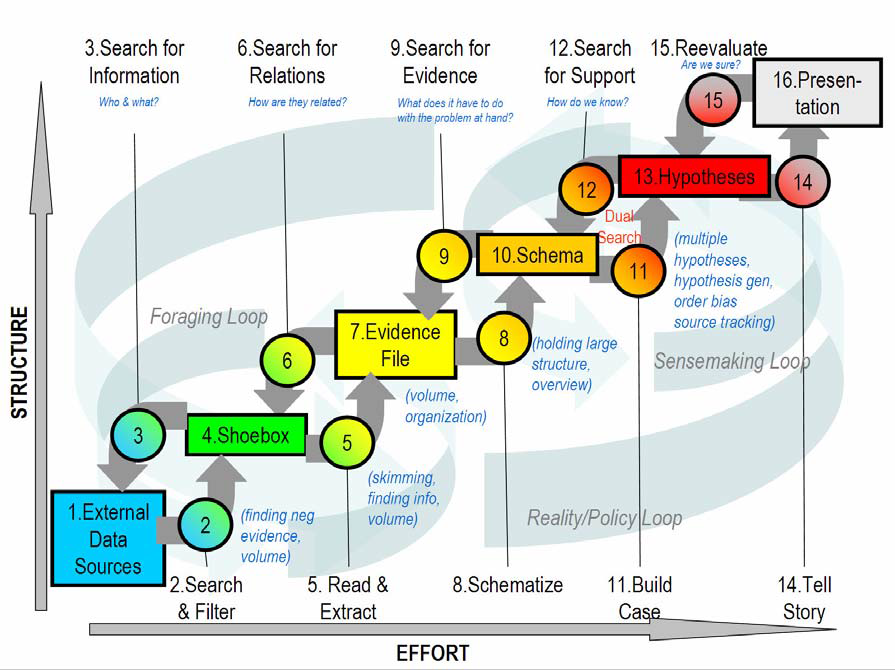
\includegraphics[width=\columnwidth]{pirolli-card-model}
	\caption{A sensemaking model proposed by Pirolli and Card. 
		\\\emph{Source: Pirolli and Card~\cite{Pirolli2005}}.}
	\label{fig:pirolli-card-model}
\end{figure}


\subsection{Data--Frame Model}
Klein et al.~\cite{Klein2003} defines sensemaking as a deliberate effort to understand an event, starting when a person realizes the gap of their current understanding of that event. These sensemaking activities are \emph{Connect data to a frame}, \emph{Elaborate a frame}, \emph{Question a frame}, \emph{Preserve a frame}, and \emph{Reframe} (Figure~\ref{fig:data-frame-model}). Sensemaking activities begin when a surprise, unexpected event with respect to our prior knowledge appears. The analyst forms an initial account for the unexpected event by connecting some evidence. In the Data-Frame model's terminology, the analyst tries to match some data to create an initial frame. When encountering new data, the analyst can either add it to the frame to elaborate the frame (if it fits to the frame) or remove existing data (if it cannot fit the frame any more). The analyst starts questioning the frame when they detect inconsistencies between data, or poor quality data in the frame. Then, they need to decide between preserving the frame by looking for more data, or reframing it by comparing it with other frames, or seeking a completely new frame. 

\begin{figure}[!htb]
	\centering
	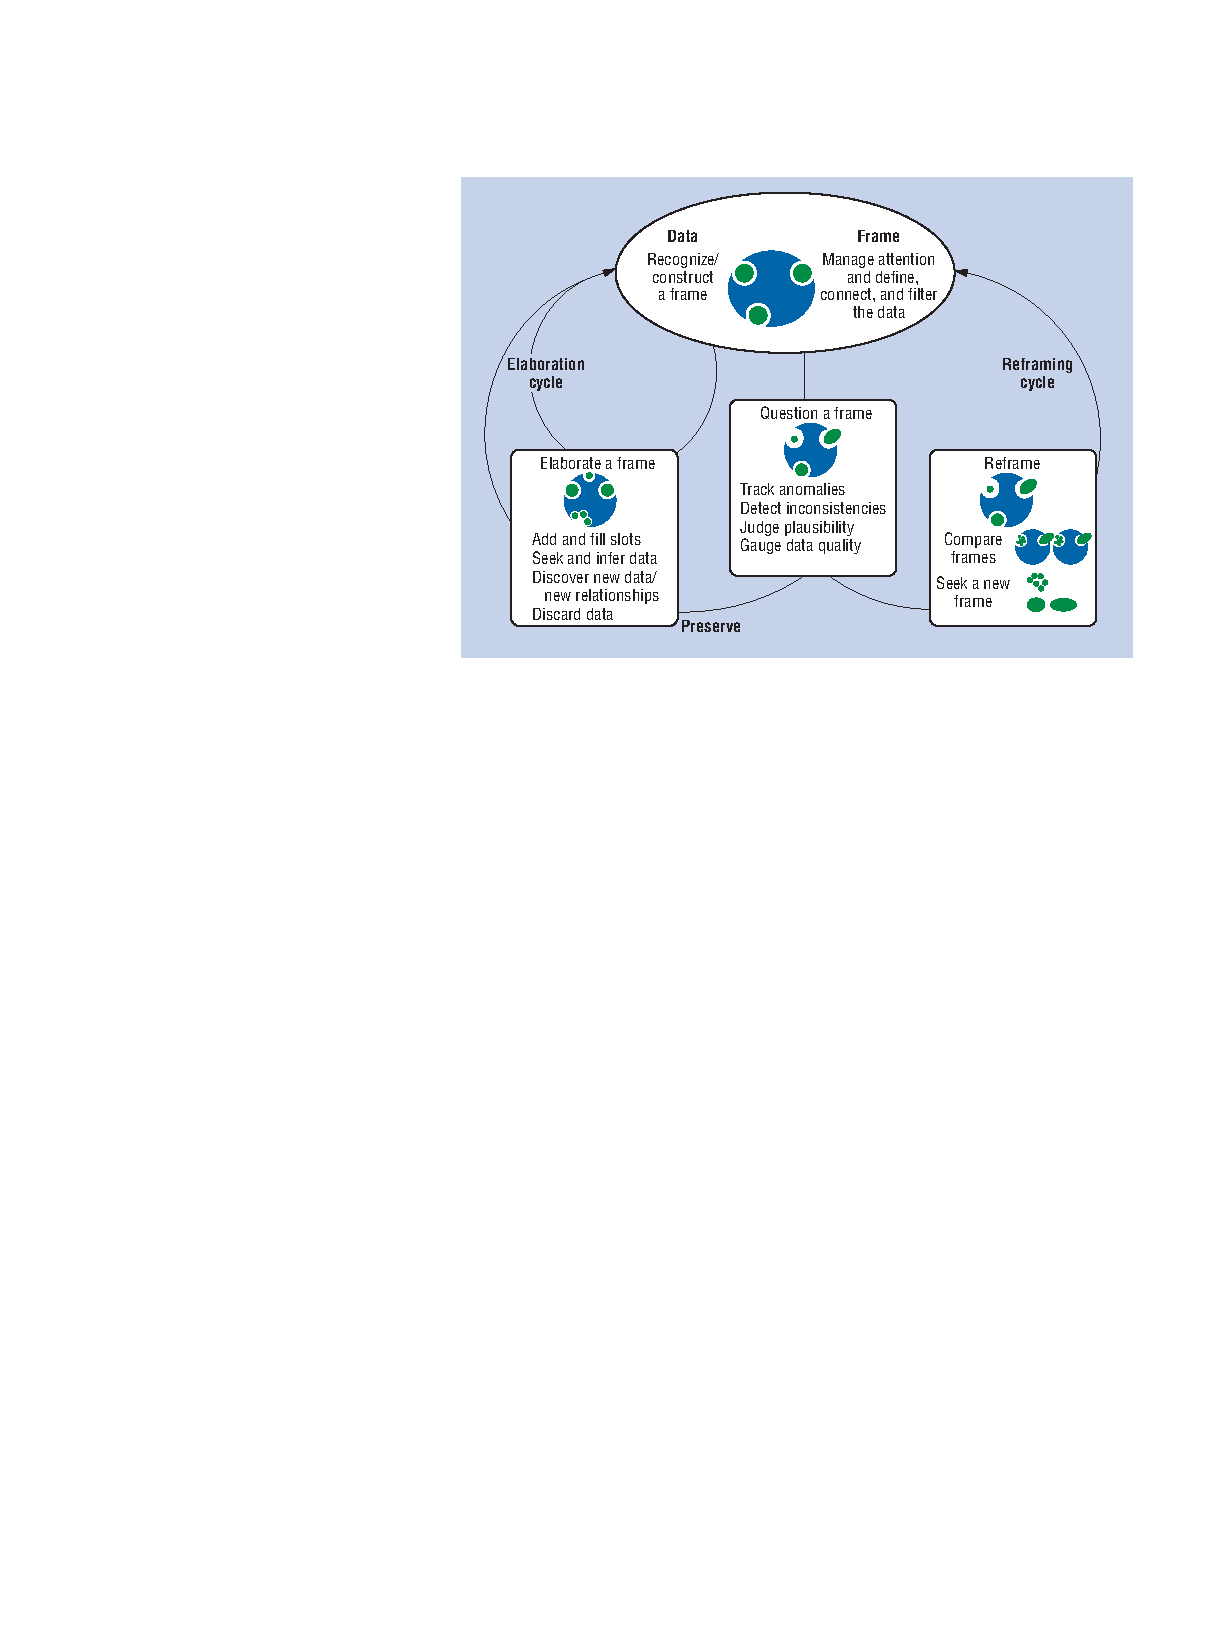
\includegraphics[width=\columnwidth]{data-frame-model}
	\caption{The data--frame model.
		\\\emph{Source: Klein et al.~\cite{Klein2003}}}
	\label{fig:data-frame-model}
\end{figure}

The Pirolli and Card's model provides a complete process model of sensemaking and identifies leverage points~\cite{Pirolli2005} that visualisation techniques can help improve. However, we find that the sensemaking loop is well elaborated through different sensemaking activities in the Data-Frame model proposed by Klein et al.~\cite{Klein2003}.